\documentclass{article}
\usepackage{amsmath,amssymb,listings,upquote}
\usepackage[margin=3cm]{geometry}
\usepackage{graphicx,color}
\lstset{language=Python}
\usepackage{enumerate}% http://ctan.org/pkg/enumerate
\usepackage{fancyvrb}


\newcounter{zone}
\setcounter{zone}{0}
\newcommand{\zone}{\clearpage\refstepcounter{zone}\section*{Zone \arabic{zone}}}
\newcounter{question}
\setcounter{question}{0}
\newcounter{variant}
\newcounter{questionpoints}
\newcommand{\question}[1]{\newpage \refstepcounter{question} \setcounter{variant}{0} \setcounter{questionpoints}{#1}}
\newcommand{\variant}{\vspace{4em}\refstepcounter{variant}\noindent \arabic{question}/\arabic{variant}. (\arabic{questionpoints} point\ifnum \thequestionpoints > 1 s\fi) }
\newenvironment{answers}{\begin{enumerate}}{\end{enumerate}}
\newcommand{\answer}{\item }
\newcommand{\correctanswer}{\item $\bigstar$ }
\renewcommand{\theenumi}{\Alph{enumi}}
\newenvironment{solution}{{\bf Solution.} }{\vspace*{.3in}\hrule}

\begin{document}

\begin{center}
\textbf{\Large CS 101 Practice Midterm \#2}
%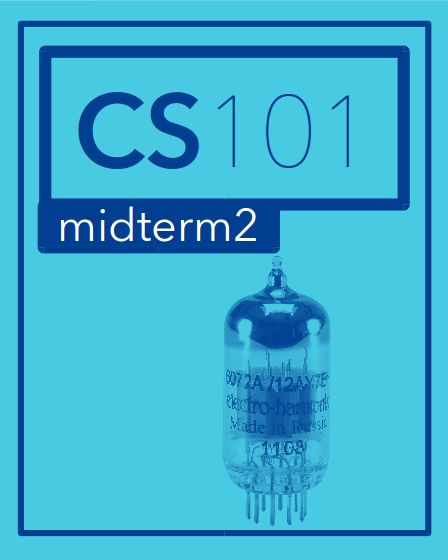
\includegraphics[width=2in]{../img/midterm2-header.png}
\end{center}

\bigskip
\noindent

\bigskip\bigskip
\noindent
\textbf{\Large 1. Fill in your information:}

\bigskip
{\Large\bf
\begin{tabular}{ll}
Full Name: & \underbar{\hskip 8cm} \\[0.5em]
UIN (Student Number): & \underbar{\hskip 8cm} \\[0.5em]
NetID: & \underbar{\hskip 8cm}
\end{tabular}
}

\bigskip
\begin{enumerate}
\item  This test is fairly representative of the contents of the second midterm.
\item  Material from lectures through \texttt{lec21} will be included.
\item  We will also test random distributions (uniform v. normal.)
\end{enumerate}

\bigskip
\noindent
\textbf{\Large 2. Fill in the following answers on the Scantron form:}

%%%%%%%%%%%%%%%%%%%%%%%%%%%%%%%%%%%%%%%%%%%%%%%%%%%%%%%%%%%%%%%%%%%%%%
%%%%%%%%%%%%%%%%%%%%%%%%%%%%%%%%%%%%%%%%%%%%%%%%%%%%%%%%%%%%%%%%%%%%%%
\zone

\question{1}
\variant
Consider the following program:
\begin{verbatim}
a=1
def f():
    return 1
    a=3
x=a+f()
\end{verbatim}
What is the \textbf{value} of x after this program is executed?
\begin{answers}
\answer \begin{verbatim}1\end{verbatim}
\correctanswer \begin{verbatim}2\end{verbatim}
\answer \begin{verbatim}3\end{verbatim}
\answer \begin{verbatim}4\end{verbatim}
\answer None of the other answers are correct.
\end{answers}
\begin{solution}
\end{solution}

%%%%%%%%%%%%%%%%%%%%%%%%%%%%%%%%%%%%%%%%%
\question{1}
\variant
Consider the following program:
\begin{verbatim}
d={}
for i,c in enumerate("ABCDEFGHIJKLMNOPQRSTUVWXYZ"):
    d[c]=i
x=0
for c in "HANSOLO":
    x+=d[c]
\end{verbatim}
What is the \textbf{value} of x after this program is executed?
\begin{answers}
\answer \begin{verbatim}84\end{verbatim}
\answer \begin{verbatim}93\end{verbatim}
\answer \begin{verbatim}62\end{verbatim}
\correctanswer \begin{verbatim}77\end{verbatim}
\answer None of the other answers are correct.
\end{answers}
\begin{solution}
\end{solution}

\question{1}
\variant
Consider the following program:
\begin{verbatim}
d={}
for i,c in enumerate("ABCDEFGHIJKLMNOPQRSTUVWXYZ"):
    d[c]=i
x=0
for c in "CHEWBACCA":
    x+=d[c]
\end{verbatim}
What is the \textbf{value} of x after this program is executed?
\begin{answers}
\answer \begin{verbatim}35\end{verbatim}
\answer \begin{verbatim}44\end{verbatim}
\answer \begin{verbatim}40\end{verbatim}
\correctanswer \begin{verbatim}77\end{verbatim}
\answer None of the other answers are correct.
\end{answers}
\begin{solution}
\end{solution}

%%%%%%%%%%%%%%%%%%%%%%%%%%%%%%%%%%%%%%%%%%%%%
\question{1}

\variant
Which of the following Python programs best simulates the roll of one six-sided die in the variable \texttt{x}?  (\emph{I.e.}, any number from 1--6 inclusive is equally likely to result from the die roll or program code.)
\begin{answers}
\correctanswer
  \begin{Verbatim}
x = np.random.choice( np.arange( 1,7 ) )
  \end{Verbatim}
\answer
  \begin{Verbatim}
x = np.random.shuffle( np.arange( 1,7 ) )
  \end{Verbatim}
\answer
  \begin{Verbatim}
x = np.random.randn( np.arange( 1,7 ) )
  \end{Verbatim}
\answer
  \begin{Verbatim}
x = np.random.uniform( np.arange( 1,7 ) )
  \end{Verbatim}
\end{answers}
\begin{solution}
\end{solution}

\question{1}
\variant
Consider the following program.
\begin{verbatim}
e=[1,2,3,4,5]
d={0:0,1:0}
for a,b in enumerate(e):
    d[b%2]+=a
x=d[1]
\end{verbatim}
After it is run, what is the final \textbf{value} of x?
\begin{answers}
\answer \begin{verbatim}3\end{verbatim}
\answer \begin{verbatim}15\end{verbatim}
\answer \begin{verbatim}4\end{verbatim}
\correctanswer \begin{verbatim}6\end{verbatim}
\answer \begin{verbatim}9\end{verbatim}
\end{answers}
\begin{solution}
\end{solution}

\question{1}
\variant
Consider the following program.
\begin{verbatim}
a=[1,"2","3",0]
x=""
for e in a:
    try:
        x+=e
    except:
        x+="A"
\end{verbatim}
After it is run, what is the final \textbf{value} of x?
\begin{answers}
\correctanswer \begin{verbatim}'A23A'\end{verbatim}
\answer \begin{verbatim}'23'\end{verbatim}
\answer \begin{verbatim}'AAAA'\end{verbatim}
\answer \begin{verbatim}'1AA0'\end{verbatim}
\answer None of the other answers are correct.
\end{answers}
\begin{solution}
\end{solution}

\question{1}
\variant
Consider the following program.
\begin{verbatim}
import numpy as np
x=np.zeros((3,3))
for i in range(3):
    x[i][i]=1
    for j in range(3):
        if i>=j:
            continue
        x[i][j]=2
\end{verbatim}
After it is run, what is the final \textbf{value} of x?
\begin{answers}
\answer $ \left[ \begin{array}{ccc} 2 & 0 & 0 \\ 2 & 2 & 0 \\ 2 & 2 & 2 \end{array} \right] $
\answer $ \left[ \begin{array}{ccc} 1 & 2 & 2 \\ 2 & 1 & 2 \\ 2 & 2 & 1 \end{array} \right] $
\answer $ \left[ \begin{array}{ccc} 1 & 0 & 0 \\ 2 & 1 & 0 \\ 2 & 2 & 1 \end{array} \right] $
\correctanswer $ \left[ \begin{array}{ccc} 1 & 2 & 2 \\ 0 & 1 & 2 \\ 0 & 0 & 1 \end{array} \right] $
\answer $ \left[ \begin{array}{ccc}  2 & 2 & 2 \\ 0 & 2 & 2 \\ 0 & 0 & 2 \end{array} \right] $
\end{answers}
\begin{solution}
\end{solution}

\question{1}
\variant
Evaluate the following expression:
\begin{verbatim}
len(",4,5,6,7".split(','))
\end{verbatim}
\begin{answers}
\answer \begin{verbatim}4\end{verbatim}
\correctanswer \begin{verbatim}5\end{verbatim}
\answer \begin{verbatim}6\end{verbatim}
\answer \begin{verbatim}22\end{verbatim}
\answer \begin{verbatim}"4567"\end{verbatim}
\end{answers}
\begin{solution}
\end{solution}

\question{1}
\variant
Consider the following program.
\begin{verbatim}
import numpy as np
x=np.array([1,2]+[3,4])+5
\end{verbatim}
After it is run, what is the final \textbf{value} of x?
\begin{answers}
\answer $ \left[ \begin{array}{cc} 6 & 7 \\ 8 & 9 \\ \end{array} \right] $
\answer $ \left[ \begin{array}{cc} 9 & 11 \\ \end{array} \right] $
\answer $ \left[ \begin{array}{c} 9 \\ 11 \\ \end{array} \right] $
\correctanswer $ \left[ \begin{array}{cccc} 6 & 7 & 8 & 9 \\ \end{array} \right] $
\answer None of the other answers are correct
\end{answers}
\begin{solution}
\end{solution}

\question{1}
\variant
Consider the following program.
\begin{verbatim}
a=list("JEDI")
for c in "EDJI":
    print(a[c])
\end{verbatim}
What kind of exception will this program throw?
\begin{answers}
\answer \begin{verbatim}KeyError: 'E'\end{verbatim}
\correctanswer \begin{verbatim}TypeError: list indices must be integers, not str\end{verbatim}
\answer \begin{verbatim}SyntaxError: invalid syntax\end{verbatim}
\answer \begin{verbatim}TypeError: cannot concatenate 'str' and 'int' objects\end{verbatim}
\answer None of the other answers are correct
\end{answers}
\begin{solution}
\end{solution}

\question{1}
\variant
Consider the following program.
\begin{verbatim}
import numpy as np
x=np.zeros((3,3))
for i in range(3):
    for j in range(3):
        x[i][j]=i*j+i
\end{verbatim}
After it is run, what is the final \textbf{value} of x?
\begin{answers}
\answer $ \left[ \begin{array}{ccc} 0 & 1 & 4 \\ 1 & 2 & 5 \\ 2 & 3 & 6 \end{array} \right] $
\answer $ \left[ \begin{array}{ccc} 0 & 1 & 2 \\ 1 & 2 & 3 \\ 4 & 5 & 6 \end{array} \right] $
\answer $ \left[ \begin{array}{ccc} 0 & 1 & 2 \\ 0 & 2 & 4 \\ 0 & 3 & 6 \end{array} \right] $
\correctanswer $ \left[ \begin{array}{ccc} 0 & 0 & 0 \\ 1 & 2 & 3 \\ 2 & 4 & 6 \end{array} \right] $
\answer None of the other answers are correct
\end{answers}
\begin{solution}
\end{solution}

%%%%%%%%%%%%%%%%%%%%%%%%%%%%%%%%%%%%%%%%%%%%%
\question{1}

\variant
For this problem, your job is to put the lines of code below in the proper order to create a function that accomplishes a task. We will completely ignore indentation.
\begin{enumerate}[1]
\item  \texttt{def is\_close( a,b,atol )}
\item  \texttt{atol = 1e-3}
\item  \texttt{return ( abs(a-b) <= atol )}
\item  \texttt{return ( (a-b) <= atol )}
\item  \texttt{except:}
\item  \texttt{def is\_close( a,b,atol=1e-3 ):}
\item  \texttt{try:}
\item  \texttt{return None}
\end{enumerate}
The function you should write is called \texttt{is\_close}, and it should accept a two numbers, \texttt{a} and \texttt{b}.  An optional third argument is the relative tolerance \texttt{atol} with default value \texttt{1e-3}.  \texttt{is\_close} \texttt{return}s \texttt{True} or \texttt{False} depending on whether the numbers are closer than \texttt{atol}:
$$
|a-b| \leq \texttt{atol} \rightarrow \texttt{True}
\hspace{3cm}
|a-b| > \texttt{atol} \rightarrow \texttt{False}
$$
The code should return \texttt{None} if the calculation fails (for instance, if the parameters \texttt{a} or \texttt{b} are non-numeric).

What is the proper selection and ordering of the given lines of code?
\begin{answers}
\correctanswer 6, 7, 3, 5, 8
\answer 6, 7, 4, 5, 8
\answer 6, 3
\answer 1, 2, 7, 4, 5, 8
\answer 1, 2, 7, 3, 5, 8
\end{answers}
\begin{solution}
\end{solution}

\question{1}
\variant
Consider the following program.
\begin{verbatim}
a,b="OBI","WAN"
def f(a):
    return tuple(a)
a,b=b,a
x=','.join(f(b))
\end{verbatim}
After it is run, what is the final \textbf{value} of x?
\begin{answers}
\correctanswer \begin{verbatim}"O,B,I"\end{verbatim}
\answer \begin{verbatim}"W,A,N"\end{verbatim}
\answer \begin{verbatim}"O","B","I"\end{verbatim}
\answer \begin{verbatim}"W","A","N"\end{verbatim}
\answer None of the other answers are correct
\end{answers}
\begin{solution}
\end{solution}

\question{1}
\variant
Consider the following program.
\begin{verbatim}
x=0
# x+=1 # x+=1
'''
'''
x+=1
'''
'''
x+=1
\end{verbatim}
After it is run, what is the final \textbf{value} of x?
\begin{answers}
\answer \begin{verbatim}1\end{verbatim}
\correctanswer \begin{verbatim}2\end{verbatim}
\answer \begin{verbatim}3\end{verbatim}
\answer \begin{verbatim}4\end{verbatim}
\answer \begin{verbatim}5\end{verbatim}
\end{answers}
\begin{solution}
\end{solution}

\question{1}
\variant
Consider the following program.
\begin{verbatim}
import numpy as np
x=np.zeros((3,3))
for i in range(3):
    for j in range(3):
        x[i][j]=i*j+j
\end{verbatim}
After it is run, what is the final \textbf{value} of x?
\begin{answers}
\answer $ \left[ \begin{array}{ccc} 0 & 1 & 4 \\ 1 & 2 & 5 \\ 2 & 3 & 6 \end{array} \right] $
\answer $ \left[ \begin{array}{ccc} 0 & 1 & 2 \\ 1 & 2 & 3 \\ 4 & 5 & 6 \end{array} \right] $
\correctanswer $ \left[ \begin{array}{ccc} 0 & 1 & 2 \\ 0 & 2 & 4 \\ 0 & 3 & 6 \end{array} \right] $
\answer $ \left[ \begin{array}{ccc} 0 & 0 & 0 \\ 1 & 2 & 3 \\ 2 & 4 & 6 \end{array} \right] $
\answer None of the other answers are correct
\end{answers}
\begin{solution}
\end{solution}

\question{1}
\variant
Consider the following program.
\begin{verbatim}
a=[1,"2","3",0]
x=""
for e in a:
    try:
        x+=int(e)
    except:
        x+="A"
\end{verbatim}
After it is run, what is the final \textbf{value} of x?
\begin{answers}
\answer \begin{verbatim}'A23A'\end{verbatim}
\answer \begin{verbatim}'23'\end{verbatim}
\correctanswer \begin{verbatim}'AAAA'\end{verbatim}
\answer \begin{verbatim}'1AA0'\end{verbatim}
\answer None of the other answers are correct.
\end{answers}
\begin{solution}
\end{solution}

%%%%%%%%%%%%%%%%%%%%%%%%%%%%%%%%%%%%%%%%%
\question{1}
\variant
Consider the following program.
\begin{verbatim}
x="5 4 1".split()
x=x.sort()
try:
    print(len(x))
except:
    print(type(x))
\end{verbatim}
After it is run, what is printed by this program?
\begin{answers}
\answer \begin{verbatim}TypeError\end{verbatim}
\answer \begin{verbatim}3\end{verbatim}
\answer \begin{verbatim}list\end{verbatim}
\correctanswer \begin{verbatim}NoneType\end{verbatim}
\end{answers}
\begin{solution}
\end{solution}

%%%%%%%%%%%%%%%%%%%%%%%%%%%%%%%%%%%%%%%%%
\question{1}
\variant
Consider the following exception.
\begin{verbatim}
ValueError: invalid literal for int() with base 10: "R"
\end{verbatim}
Which of the following programs will throw this exception?
\begin{answers}
\correctanswer \begin{verbatim}int("RANCOR"[0])\end{verbatim}
\answer \begin{verbatim}10+"RANCOR"\end{verbatim}
\answer \begin{verbatim}"RAN"[10]"COR"\end{verbatim}
\answer \begin{verbatim}"RANCOR"[int("10")]\end{verbatim}
\answer None of the other answers are correct
\end{answers}
\begin{solution}
\end{solution}
\question{1}
\variant
Consider the following exception.
\begin{verbatim}
TypeError: can only concatenate tuple (not "int") to tuple
\end{verbatim}
Which of the following programs will throw this exception?
\begin{answers}
\correctanswer \begin{verbatim}tuple("LAN")+len("DO")\end{verbatim}
\answer \begin{verbatim}tuple("LAN")[len("DO")]\end{verbatim}
\answer \begin{verbatim}tuple("LAN")+tuple("DO")\end{verbatim}
\answer \begin{verbatim}"LAN"+[tuple("DO")]\end{verbatim}
\answer None of the other answers are correct
\end{answers}
\begin{solution}
\end{solution}

\question{1}
\variant
Consider the following 2-dimensional numpy array:

$ \left[ \begin{array}{ccc} 1 & 5 & 9 \\ 2 & 6 & 10 \\ 3 & 7 & 11 \\ 4 & 8 & 12 \\ \end{array} \right] $ \\

Assuming it is stored in a variable named a, how can we index and retrieve the value 7?
\begin{answers}
\answer a[1][2]
\correctanswer a[2][1]
\answer a[2][3]
\answer a[3][2]
\end{answers}
\begin{solution}
\end{solution}

\question{1}
\variant
Consider the following program.
\begin{verbatim}
def f(x):
    for i in range(x):
        return x+1
    return 100
x=f(5)
\end{verbatim}
After it is run, what is the final \textbf{value} of x?
\begin{answers}
\answer \begin{verbatim}6\end{verbatim}
\answer \begin{verbatim}3\end{verbatim}
\answer \begin{verbatim}5\end{verbatim}
\answer \begin{verbatim}100\end{verbatim}
\correctanswer None of the other answers are correct.
\end{answers}
\begin{solution}
\end{solution}

\question{1}
\variant
Consider the following program.
\begin{verbatim}
def f(x):
    if x<10:
       print(x)
   else:
       print(x+1)
x=f(5)
\end{verbatim}
After it is run, what is the final \textbf{value} of x?
\begin{answers}
\answer \begin{verbatim}4\end{verbatim}
\answer \begin{verbatim}10\end{verbatim}
\answer \begin{verbatim}5\end{verbatim}
\answer \begin{verbatim}6\end{verbatim}
\correctanswer None of the other answers are correct.
\end{answers}
\begin{solution}
\end{solution}
\question{1}
\variant
Consider the following incomplete function.
\begin{verbatim}
def pal(s):
    a=list(s)
    n=len(s)
    ???
\end{verbatim}
The function is intended to return True if and only if the input string s is a palindrome. A palindrome is a string that reads the same forward and backward, like ``ABBA'' or ``RACECAR''. What should replace the three question marks to complete the function?
\begin{answers}
\answer  \begin{verbatim}return a==a.reverse() \end{verbatim}
\answer  \begin{verbatim}return a[:n/2]==a[(n+1)/2:] \end{verbatim}
\correctanswer
\begin{verbatim}for i in range(n):
    if a[i]!=a[n-i-1]:
        return False
return True
\end{verbatim}
\answer  \begin{verbatim}return a[0:n:-1]==a[n:0:1] \end{verbatim}
\answer  \begin{verbatim}None of the other answers are correct. \end{verbatim}
\end{answers}
\begin{solution}
\end{solution}
\question{1}
\variant
Consider the following program.
\begin{verbatim}
x=[]
for j in range(0,6):
    if (j%4)==0:
        x.append("-")
    if (j%3)==0:
        x.append("*")
\end{verbatim}
After it is run, what is the final \textbf{value} of x?
\begin{answers}
\answer \begin{verbatim}["-","*"]\end{verbatim}
\answer \begin{verbatim}["*","-","*"]\end{verbatim}
\answer \begin{verbatim}["*","-","*"]\end{verbatim}
\correctanswer \begin{verbatim}["-","*","*","-"]\end{verbatim}
\answer None of the other answers are correct.
\end{answers}
\begin{solution}
\end{solution}
\question{1}
\variant
Consider the following Python program.
\begin{verbatim}
e=list(range(6,-1,-1))
d={0:1,1:2,2:3,3:4}
for i in e:
    d[i%3]+=e[i]
x=d[1]
\end{verbatim}
After it is run, what is the final \textbf{value} of x?
\begin{answers}
\answer \begin{verbatim}3\end{verbatim}
\answer \begin{verbatim}5\end{verbatim}
\answer \begin{verbatim}16\end{verbatim}
\answer \begin{verbatim}12\end{verbatim}
\correctanswer \begin{verbatim}9\end{verbatim}
\end{answers}
\begin{solution}
\end{solution}


%%%%%%%%%%%%%%%%%%%%%%%%%%%%%%%%%%%%%%%%%%%%%
\question{1}
\variant
Consider the following program.  (N.B.:  This is a tricky one!)
\begin{Verbatim}
def chase( chevy ):
    chevy.append( "arrow" )
    chevy.reverse()
    chevy = chevy.sort()
    return chevy

earl = "cheviot hills".split(" ")
chase( earl )
\end{Verbatim}
After it is run, what is the final \textbf{value} of \texttt{earl}?
\begin{answers}
\answer \texttt{[ 'hills', 'cheviot', 'arrow' ]}
\correctanswer \texttt{[ 'arrow', 'cheviot', 'hills' ]}
\answer \texttt{None}
\answer \texttt{[ 'hills', 'cheviot' ]}
\answer \texttt{[ 'cheviot', 'hills', 'arrow' ]}
\end{answers}
\begin{solution}
\end{solution}

\question{1}
\variant
What should replace the three question marks to produce a program that runs without throwing an exception? Note: \texttt{sin}, \texttt{cos}, and \texttt{pi} are all part of the \texttt{math} module.
\begin{verbatim}
???
math.sin(pi)+math.cos(pi)
\end{verbatim}
\begin{answers}
\answer \begin{verbatim}from math import sin,cos
import math
\end{verbatim}
\answer \begin{verbatim}from math import *
import sin,cos
\end{verbatim}
\correctanswer \begin{verbatim}import math
from math import pi
\end{verbatim}
\answer \begin{verbatim}import math as pi, as sin, as cos\end{verbatim}
\end{answers}
\begin{solution}
\end{solution}

%%%%%%%%%%%%%%%%%%%%%%%%%%%%%%%%%%%%%%%%%%%%%
\question{1}

\variant
Consider the following incomplete Python program:
\begin{Verbatim}
def tribo( n ):
    if n <= 1:
        return 1
    else:
        ???
\end{Verbatim}
The function \texttt{tribo} should return the $n$th number of the so-called ``Tribonacci'' sequence (counting from zero), in which each number is equal to the sum of the preceding three; \emph{i.e.},
$$
0,\,0,\,1,\,1,\,2,\,4,\,7,\,13,\,24,\,44,\,81,\,...
$$
What should replace the \texttt{???} block to complete the program correctly?
\begin{answers}
\correctanswer \texttt{return tribo( n-1 ) + tribo( n-2 ) + tribo( n-3 )}
\answer \texttt{return tribo( n ) + tribo( n-1 ) + tribo( n-2 )}
\answer \texttt{return tribo( n-1, n-2, n-3 )}
\answer \texttt{return (n - 1) + (n - 2) + (n - 3)}
\answer \texttt{return tribo[ n-1 ] + tribo[ n-2 ] + tribo[ n-3 ]}
\end{answers}
\begin{solution}
\end{solution}

\end{document}
